\documentclass[11pt]{article}
\usepackage{amsmath, textcomp, amssymb, geometry, graphicx, enumerate, ctex, float}
\usepackage[colorlinks, linkcolor=black]{hyperref}
\usepackage{listings}		% 为了避免与页眉的兼容问题可将listings放入table环境中
\lstset{
    basicstyle          =   \sffamily,          % 基本代码风格
    keywordstyle        =   \color{blue},          % 关键字风格
    keywordstyle    =   [2] \color{teal},
    commentstyle        =   \rmfamily\itshape,  % 注释的风格,斜体
    stringstyle         =   \ttfamily,  % 字符串风格
    flexiblecolumns,                % 别问为什么,加上这个
    numbers             =   left,   % 行号的位置在左边
    showspaces          =   false,  % 是否显示空格,显示了有点乱,所以不现实了
    numberstyle         =   \zihao{-5}\ttfamily,    % 行号的样式,小五号,tt等宽字体
    showstringspaces    =   false,
    captionpos          =   t,      % 这段代码的名字所呈现的位置,t指的是top上面
    frame               =   lrtb,   % 显示边框
    basicstyle          =   \zihao{-5}\ttfamily,
    stringstyle         =   \color{magenta},
    commentstyle        =   \color{red}\ttfamily,
    breaklines          =   true,   % 自动换行,建议不要写太长的行
    columns             =   fixed,  % 如果不加这一句,字间距就不固定,很丑,必须加
    basewidth           =   0.5em,
}
\geometry{left=2.54cm, right=2.54cm, top=3.18cm, bottom=3.18cm}

\def\Name{杨豪\space}  % Your name
\def\SID{2206213297}  % Your student ID number

% need to be confirmed before each time writing and committing 
\def\Homework{3} % Number of Homework
\def\Session{2022-Fall}
\def\CourseCodeName{SOFT400227: Operating System}
\def\simCourseName{OS}

\title{\vspace{-4cm}\CourseCodeName \space
        \Session \protect\\  Homework-\textbf{\Homework} Solutions}
\author{软件2101 \Name \space 学号: \SID}
\markright{\simCourseName\ \space \Session\  HW-\Homework\ \Name}
\date{\today}


\begin{document}
\maketitle
\vspace{-0.8cm}
\textbf{Honor Code: I promise that I finished the homework solutions on my own without copying other people's 
    work.}

\section*{Scheduler}

\subsection*{1. }

A CPU-bound program spends most of its time executing instructions on the processor while a I/O-bound program spends 
most of its time waiting for input and output operations to complete. 

Distinguishing them is helpful for scheduling processes to utilize CPU better. 

\subsection*{2. }

use N-Pir as a short case for non-preemptive priority

\subsubsection*{a. Gantt charts}

\begin{figure}[H]
    \centering
    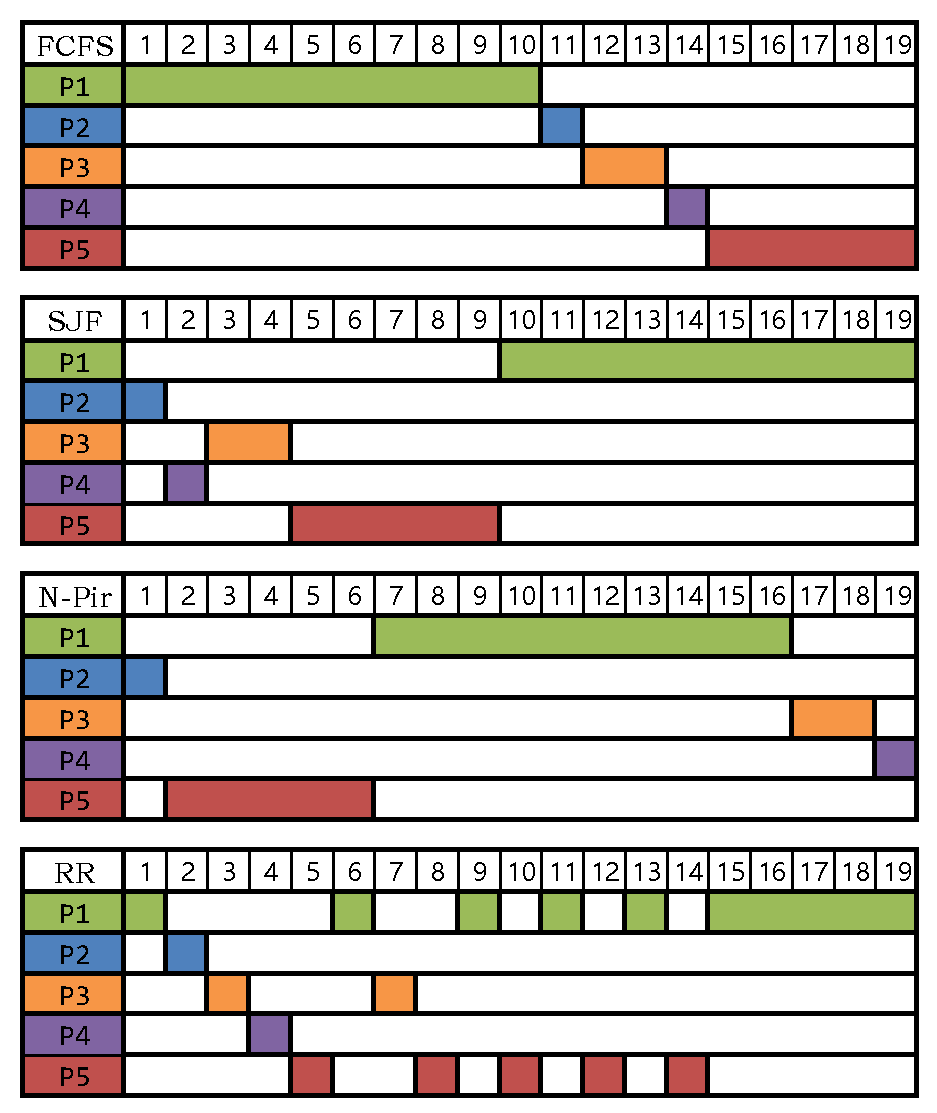
\includegraphics[width = 0.5\textwidth]{pic/gant.pdf}
\end{figure}

\subsubsection*{b. }
% What is the turnaround time of each process for each of the scheduling algorithms in part a?

\begin{table}[H]
    \centering
    \begin{tabular}{|c|c|c|c|c|}
        \hline
                        & \textbf{FCFS} & \textbf{SJF} & \textbf{N-Pir} & \textbf{RR} \\ \hline
        \textbf{turnaround time} & 13.4          & 7            & 12             & 9.2         \\ \hline
    \end{tabular}
\end{table}

\begin{itemize}
    \item[FCFS.] $t_1 = (10+11+13+14+19)/5=13.4$
    \item[SJF.] $t_2 = (19+1+4+2+9)/5=7$
    \item[N-Pir.] $t_3 = (16+1+18+19+6)/5=12 $ 
    \item[RR.] $t_4 = (19+2+7+4+14)/5=9.2$
\end{itemize}

\subsection*{c.\&d.}
\begin{table}[H]
    \centering
    \begin{tabular}{|c|c|c|c|c|}
        \hline
        \textbf{Waiting time} & \textbf{FCFS} & \textbf{SJF} & \textbf{N-Pir} & \textbf{RR} \\ \hline
        \textbf{P1}          & 0             & 9            & 6              & 9           \\ \hline
        \textbf{P2}          & 10            & 0            & 0              & 1           \\ \hline
        \textbf{P3}          & 11            & 2            & 16             & 5           \\ \hline
        \textbf{P4}          & 13            & 1            & 18             & 3           \\ \hline
        \textbf{P5}          & 14            & 4            & 1              & 9           \\ \hline
        \textbf{Average}     & 9.6           & 3.2          & 8.2            & 5.4         \\ \hline
    \end{tabular}
\end{table}
minimum average waiting time: SJF

\subsection*{3. }
Answer: \textbf{b}, \textbf{d}

\begin{enumerate}
    \item[b.] When a long job waiting for a lot of short jobs.
    \item[d.] When a low priority job waiting for a lot of high priority jobs.
\end{enumerate}

\subsection*{4. }


\begin{table}[H]
    \centering
    \begin{tabular}{|c|c|c|c|}
    \hline
    \textbf{}         & \textbf{P1} & \textbf{P2} & \textbf{P3} \\ \hline
    \textbf{Priority} & 80          & 69          & 65          \\ \hline
    \end{tabular}
\end{table}

 
    Will lower the relative priority of a CPU-bound process. 
    
    CPU-bound don't need to wait for 
    I/O and finish their tasks on CPU, so they use CPU less frequently than I/O.


% they also need to be checked.
\section*{Other things}

    \LaTeX \space code refer to these things and was complied on texlive2020.
    \begin{itemize}
        \item  \href{https://www.eecs70.org/assets/misc/homework_template.tex}{UCB-CS70's given homework template.} 
        \item  \href{https://www.latexlive.com}{A free website useful to edit \LaTeX \space formula code.}
        \item  \href{https://www.tablesgenerator.com/}{A free website helpful to generate \LaTeX \space table.}
    \end{itemize}

    Some description refer to \textit{Operating System Concepts 10th}, \href{https://en.wikipedia.org}{Wikipedia} and Professor.Tian's PPT.

    The purpose of writing in English is to adapt to bilingual teaching and to improve my poor English 
    writing skills in preparation for a possible future exchange program. 

    Thanks for your correcting and grading :).

\end{document}